%%%%%%%%%%%%%%%%%%%%%%%%%%%%%%%%%%%%%%%%%%%%%%%%%%%%%%%%%%%%%%%%%%%%%%%%%%%%%%%%%%
\begin{frame}[fragile]\frametitle{}
\begin{center}
{\Large Logistic Regression - Alice}

{\tiny (Ref: mlcourse.ai Assignment 4 – Open Machine Learning Course ) }
\end{center}

https://mlcourse.ai/notebooks/blob/master/jupyter\_english/assignments\_fall2018/assignment4\_websites\_logistic\_regression.ipynb

https://www.youtube.com/watch?v=7o0SWgY89i8

\end{frame}


%%%%%%%%%%%%%%%%%%%%%%%%%%%%%%%%%%%%%%%%%%%%%%%%%%%%%%%%%%
\begin{frame}[fragile]\frametitle{Problem Info}
User Identification with Logistic Regression	
\begin{itemize}
\item Kaggle In class Competition : https://www.kaggle.com/c/catch-me-if-you-can-intruder-detection-through-webpage-session-tracking2
\item We''ll analyze the sequence of websites consequently visited by a particular person and try to predict whether this person is Alice or someone else. As a metric we will use ROC AUC.
\item Download data from https://inclass.kaggle.com/c/catch-me-if-you-can-intruder-detection-through-webpage-session-tracking2
\end{itemize}
\end{frame}



%%%%%%%%%%%%%%%%%%%%%%%%%%%%%%%%%%%%%%%%%%%%%%%%%%%%%%%%%%
\begin{frame}[fragile]\frametitle{Import Libraries}
\begin{lstlisting}
import pickle
import numpy as np
import pandas as pd
from scipy.sparse import csr_matrix, hstack
from sklearn.preprocessing import StandardScaler
from sklearn.metrics import roc_auc_score
from sklearn.linear_model import LogisticRegression
from matplotlib import pyplot as plt
import seaborn as sns
sns.set()
\end{lstlisting}
\end{frame}

%%%%%%%%%%%%%%%%%%%%%%%%%%%%%%%%%%%%%%%%%%%%%%%%%%%%%%%%%%
\begin{frame}[fragile]\frametitle{Read Data}	
\begin{lstlisting}
train_df = pd.read_csv('data/train_sessions.csv',index_col='session_id')
test_df = pd.read_csv('data/test_sessions.csv',index_col='session_id')

# Convert time1, ..., time10 columns to datetime type
times = ['time%s' % i for i in range(1, 11)]
train_df[times] = train_df[times].apply(pd.to_datetime)
test_df[times] = test_df[times].apply(pd.to_datetime)

train_df = train_df.sort_values(by='time1')
train_df.head() 
\end{lstlisting}
\begin{center}
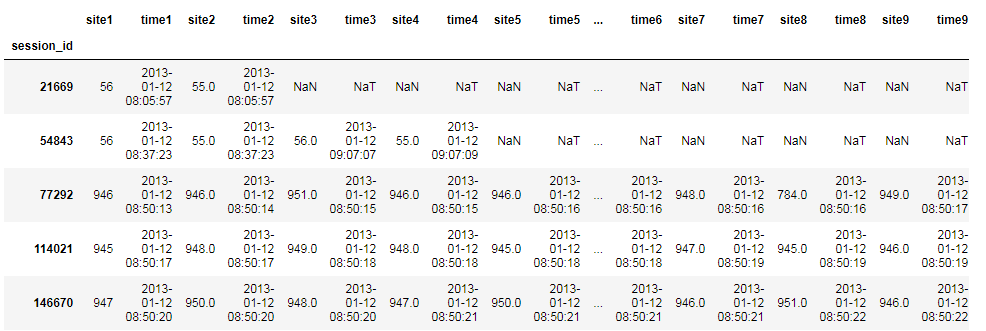
\includegraphics[width=0.8\linewidth,keepaspectratio]{logreg6}
\end{center}
\end{frame}


%%%%%%%%%%%%%%%%%%%%%%%%%%%%%%%%%%%%%%%%%%%%%%%%%%%%%%%%%%
\begin{frame}[fragile]\frametitle{Features}
The training data set contains the following features:
\begin{itemize}
\item site1 – id of the first visited website in the session
\item time1 – visiting time for the first website in the session
\item \ldots
\item site10 – id of the tenth visited website in the session
\item time10 – visiting time for the tenth website in the session
\item target – target variable, 1 for Alice's sessions, and 0 for the other users' sessions
\end{itemize}
\end{frame}

%%%%%%%%%%%%%%%%%%%%%%%%%%%%%%%%%%%%%%%%%%%%%%%%%%%%%%%%%%
\begin{frame}[fragile]\frametitle{Input information}
\begin{itemize}
\item User sessions are chosen in the way that they are shorter than 30 minutes and contain no more than 10 websites. 
\item i.e. a session is considered over either if a user has visited 10 websites or if a session has lasted over 30 minutes.

\item There are some empty values in the table, it means that some sessions contain less than ten websites. 
\end{itemize}
\end{frame}

%%%%%%%%%%%%%%%%%%%%%%%%%%%%%%%%%%%%%%%%%%%%%%%%%%%%%%%%%%
\begin{frame}[fragile]\frametitle{Transform Data}	
Replace empty values with 0 and change columns types to integer. Also load the websites dictionary and check how it looks like:
\begin{lstlisting}
# Change site1, ..., site10 columns type to integer and fill NA-values with zeros
sites = ['site%s' % i for i in range(1, 11)]
train_df[sites] = train_df[sites].fillna(0).astype(np.uint16)
test_df[sites] = test_df[sites].fillna(0).astype(np.uint16)

# Load websites dictionary
with open(r"data/site_dic.pkl", "rb") as input_file:
    site_dict = pickle.load(input_file)

sites_dict = pd.DataFrame(list(site_dict.keys()), index=list(site_dict.values()), columns=['site'])
print(u'Websites total:', sites_dict.shape[0])
>> Websites total: 48371
sites_dict.head()
\end{lstlisting}
\begin{center}
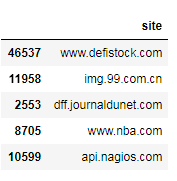
\includegraphics[width=0.15\linewidth,keepaspectratio]{logreg7}
\end{center}
\end{frame}

%%%%%%%%%%%%%%%%%%%%%%%%%%%%%%%%%%%%%%%%%%%%%%%%%%%%%%%%%%
\begin{frame}[fragile]\frametitle{Question 1}
What are the dimensions of the training and test sets (in exactly this order)?
\begin{itemize}
\item (82797, 20) and (253561, 20)
\item (82797, 20) and (253561, 21)
\item (253561, 21) and (82797, 20)
\item (253561, 20) and (82797, 20)
\end{itemize}
Answer XX
\end{frame}

%%%%%%%%%%%%%%%%%%%%%%%%%%%%%%%%%%%%%%%%%%%%%%%%%%%%%%%%%%
\begin{frame}[fragile]\frametitle{Brief Exploratory Data Analysis}	
\begin{lstlisting}
# Top websites in the training data set
top_sites = pd.Series(train_df[sites].values.flatten()
                     ).value_counts().sort_values(ascending=False).head(5)
print(top_sites)
sites_dict.loc[top_sites.drop(0).index]
>>
21     123776
0      122730
23      87619
782     77055
22      58258
dtype: int64
\end{lstlisting}
\begin{center}
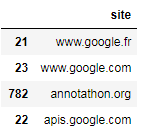
\includegraphics[width=0.15\linewidth,keepaspectratio]{logreg8}
\end{center}
\end{frame}

%%%%%%%%%%%%%%%%%%%%%%%%%%%%%%%%%%%%%%%%%%%%%%%%%%%%%%%%%%
\begin{frame}[fragile]\frametitle{Question 2}
What kind of websites does Alice visit the most?
\begin{itemize}
\item videohostings
\item social networks
\item torrent trackers
\item news
\end{itemize}
Answer XX
\end{frame}


%%%%%%%%%%%%%%%%%%%%%%%%%%%%%%%%%%%%%%%%%%%%%%%%%%%%%%%%%%
\begin{frame}[fragile]\frametitle{Brief Exploratory Data Analysis}	
Now let us look at the timestamps and try to characterize sessions as timeframes:
\begin{lstlisting}
# Create a separate dataframe where we will work with timestamps
time_df = pd.DataFrame(index=train_df.index)
time_df['target'] = train_df['target']

# Find sessions' starting and ending
time_df['min'] = train_df[times].min(axis=1)
time_df['max'] = train_df[times].max(axis=1)

# Calculate sessions' duration in seconds
time_df['seconds'] = (time_df['max'] - time_df['min']) / np.timedelta64(1, 's')

time_df.head()
\end{lstlisting}
\begin{center}
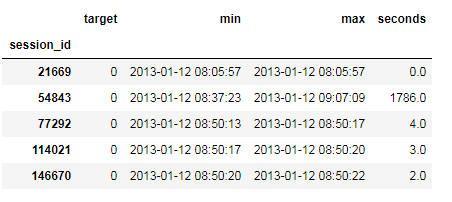
\includegraphics[width=0.5\linewidth,keepaspectratio]{logreg9}
\end{center}
\end{frame}

%%%%%%%%%%%%%%%%%%%%%%%%%%%%%%%%%%%%%%%%%%%%%%%%%%%%%%%%%%
\begin{frame}[fragile]\frametitle{Question 2}
Select all correct statements:
\begin{itemize}
\item On average, Alice's session is shorter than that of other users
\item More than 1\% of all sessions in the dataset belong to Alice
\item Minimum and maximum durations of Alice's and other users' sessions are approximately the same
\item Variation about the mean session duration for all users (including Alice) is approximately the same
\item Less than a quarter of Alice's sessions are greater than or equal to 40 seconds
\end{itemize}
Answer XX
\end{frame}

%%%%%%%%%%%%%%%%%%%%%%%%%%%%%%%%%%%%%%%%%%%%%%%%%%%%%%%%%%
\begin{frame}[fragile]\frametitle{Prepare Data for Training}	
\begin{itemize}
\item First of all, exclude the target variable from the training set. 
\item Now both training and test sets have the same number of columns, therefore aggregate them into one dataframe. 
\item Thus, all transformations will be performed simultaneously on both training and test data sets.
\end{itemize}
\begin{lstlisting}
# Our target variable
y_train = train_df['target']

# United dataframe of the initial data 
full_df = pd.concat([train_df.drop('target', axis=1), test_df])

# Index to split the training and test data sets
idx_split = train_df.shape[0]
\end{lstlisting}
\end{frame}

%%%%%%%%%%%%%%%%%%%%%%%%%%%%%%%%%%%%%%%%%%%%%%%%%%%%%%%%%%
\begin{frame}[fragile]\frametitle{Prepare Data for Training}	
\begin{itemize}
\item For the very basic model, we will use only the visited websites in the session (but we will not take into account timestamp features). 
\item The point behind this data selection is: Alice has her favorite sites, and the more often you see these sites in the session, the higher probability that this is Alice's session, and vice versa.
\item We will take only features $site1, site2, \ldots , site10$ from the whole dataframe. 
\item Keep in mind that the missing values are replaced with zero.
\end{itemize}
\end{frame}

%%%%%%%%%%%%%%%%%%%%%%%%%%%%%%%%%%%%%%%%%%%%%%%%%%%%%%%%%%
\begin{frame}[fragile]\frametitle{Prepare Data for Training}	
Here is how the first rows of the dataframe look like:
\begin{lstlisting}
# Dataframe with indices of visited websites in session
full_sites = full_df[sites]
full_sites.head()
\end{lstlisting}

\begin{center}
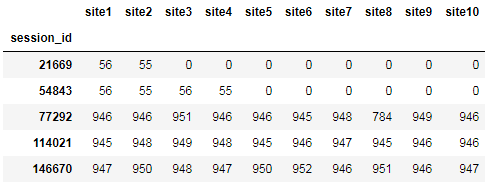
\includegraphics[width=0.5\linewidth,keepaspectratio]{logreg10}
\end{center}

Sessions are sequences of website indices, and data in this representation is useless for machine learning method (just think, what happens if we switched all ids of all websites).
\end{frame}


%%%%%%%%%%%%%%%%%%%%%%%%%%%%%%%%%%%%%%%%%%%%%%%%%%%%%%%%%%
\begin{frame}[fragile]\frametitle{Prepare Data for Training}	
According to our hypothesis (Alice has favorite websites), we need to transform this dataframe so each website has a corresponding feature (column) and its value is equal to number of this website visits in the session.
\begin{lstlisting}
# sequence of indices
sites_flatten = full_sites.values.flatten()

full_sites_sparse = csr_matrix(([1] * sites_flatten.shape[0],
    sites_flatten,range(0, sites_flatten.shape[0]  + 10, 10)))[:, 1:]

full_sites_sparse.shape
>>>
(336358, 48371)
\end{lstlisting}
More on Sparse Matrices, next \ldots
\end{frame}

%%%%%%%%%%%%%%%%%%%%%%%%%%%%%%%%%%%%%%%%%%%%%%%%%%%%%%%%%%
\begin{frame}[fragile]\frametitle{Important detour \#1: Sparse Matrices}	
\begin{itemize}
\item Let us estimate how much memory it will require to store our data in the example above. 
\item Our united dataframe contains 336 thousand samples of 48 thousand integer features in each. 
\item It's easy to calculate the required amount of memory, roughly:
$336K * 48K * 8 bytes = 16M * 8 bytes = 128 GB,$

\item It will not be easy to do anything with it.
\item Imp observation: most of the elements of our matrix are zeros, about 90\%
\item This matrix is called sparse, and the ratio between the number of zero elements and the total number of elements is called the sparseness of the matrix.
\end{itemize}

\end{frame}

%%%%%%%%%%%%%%%%%%%%%%%%%%%%%%%%%%%%%%%%%%%%%%%%%%%%%%%%%%
\begin{frame}[fragile]\frametitle{Important detour \#1: Sparse Matrices}	
For the work with such matrices you can use scipy.sparse library
\begin{lstlisting}
# How much memory does a sparse matrix occupy?
print('{0} elements * {1} bytes = {2} bytes'.format(full_sites_sparse.count_nonzero(), 8, 
                                                    full_sites_sparse.count_nonzero() * 8))
# Or just like this:
print('sparse_matrix_size = {0} bytes'.format(full_sites_sparse.data.nbytes))

>>>
1866898 elements * 8 bytes = 14935184 bytes
sparse_matrix_size = 14935184 bytes
\end{lstlisting}

\end{frame}

%%%%%%%%%%%%%%%%%%%%%%%%%%%%%%%%%%%%%%%%%%%%%%%%%%%%%%%%%%
\begin{frame}[fragile]\frametitle{Important detour \#1: Sparse Matrices}	
Let us explore how the matrix with the websites has been formed using a mini example. Suppose we have the following table with user sessions:

\begin{center}
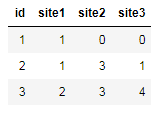
\includegraphics[width=0.3\linewidth,keepaspectratio]{logreg11}
\end{center}

There are 3 sessions, and no more than 3 websites in each. Users visited four different sites in total (there are numbers from 1 to 4 in the table cells). And let us assume that the mapping is:

\begin{itemize}
\item vk.com
\item habrahabr.ru
\item yandex.ru
\item ods.ai
\end{itemize}
\end{frame}

%%%%%%%%%%%%%%%%%%%%%%%%%%%%%%%%%%%%%%%%%%%%%%%%%%%%%%%%%%
\begin{frame}[fragile]\frametitle{Important detour \#1: Sparse Matrices}	
\begin{itemize}
\item If the user has visited less than 3 websites during the session, the last few values will be zero. \item We want to convert the original dataframe in a way that each session has a corresponding row which shows the number of visits to each particular site. I.e. we want to transform the previous table into the following form:
\end{itemize}

\begin{center}
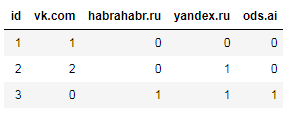
\includegraphics[width=0.5\linewidth,keepaspectratio]{logreg12}
\end{center}
\end{frame}

%%%%%%%%%%%%%%%%%%%%%%%%%%%%%%%%%%%%%%%%%%%%%%%%%%%%%%%%%%
\begin{frame}[fragile]\frametitle{Important detour \#1: Sparse Matrices}	
\begin{itemize}
\item To do this, use the constructor: csr\_matrix ((data, indices, indptr)) and create a frequency table 
\item Here we set all the parameters explicitly for greater clarity:
\end{itemize}

\begin{lstlisting}
# data, create the list of ones, length of which equal to the number of elements in the initial dataframe (9)
# By summing the number of ones in the cell, we get the frequency,
# number of visits to a particular site per session
data = [1] * 9

# To do this, you need to correctly distribute the ones in cells
# Indices - website ids, i.e. columns of a new matrix. We will sum ones up grouping them by sessions (ids)
indices = [1, 0, 0, 1, 3, 1, 2, 3, 4]

# Indices for the division into rows (sessions)
# For example, line 0 is the elements between the indices [0; 3) - the rightmost value is not included
# Line 1 is the elements between the indices [3; 6)
# Line 2 is the elements between the indices [6; 9) 
indptr = [0, 3, 6, 9]
\end{lstlisting}

\end{frame}


%%%%%%%%%%%%%%%%%%%%%%%%%%%%%%%%%%%%%%%%%%%%%%%%%%%%%%%%%%
\begin{frame}[fragile]\frametitle{Important detour \#1: Sparse Matrices}	
\begin{lstlisting}
# Aggregate these three variables into a tuple and compose a matrix
# To display this matrix on the screen transform it into the usual "dense" matrix
csr_matrix((data, indices, indptr)).todense()

>>>
matrix([[2, 1, 0, 0, 0],
        [0, 2, 0, 1, 0],
        [0, 0, 1, 1, 1]])
\end{lstlisting}

\begin{itemize}
\item As you might have noticed, there are not four columns in the resulting matrix (corresponding to number of different websites) but five. A zero column has been added, which indicates if the session was shorter (in our mini example we took sessions of three). 
\item This column is excessive and should be removed from the dataframe (do that yourself).
\end{itemize}

\end{frame}

%%%%%%%%%%%%%%%%%%%%%%%%%%%%%%%%%%%%%%%%%%%%%%%%%%%%%%%%%%
\begin{frame}[fragile]\frametitle{Question 4}
What is the sparseness of the matrix in our small example?
\begin{itemize}
\item 42\%
\item 47\%
\item 50\%
\item 53\%
\end{itemize}
Answer XX
\end{frame}

%%%%%%%%%%%%%%%%%%%%%%%%%%%%%%%%%%%%%%%%%%%%%%%%%%%%%%%%%%
\begin{frame}[fragile]\frametitle{Important detour \#1: Sparse Matrices}	
\begin{itemize}
\item Another benefit of using sparse matrices is that there are special implementations of both matrix operations and machine learning algorithms for them, which sometimes allows to significantly accelerate operations due to the data structure peculiarities. 
\item This applies to logistic regression as well. 
\item Now everything is ready to build our first model.
\end{itemize}

\end{frame}

%%%%%%%%%%%%%%%%%%%%%%%%%%%%%%%%%%%%%%%%%%%%%%%%%%%%%%%%%%
\begin{frame}[fragile]\frametitle{Training the first model}	
We will use the first 90\% of the data for training (the training data set is sorted by time), and the remaining 10\% for validation.  Let's write a simple function that returns the quality of the model and then train our first classifier:

\begin{lstlisting}
def get_auc_lr_valid(X, y, C=1.0, seed=17, ratio = 0.9):
    # Split the data into the training and validation sets
    idx = int(round(X.shape[0] * ratio))
    # Classifier training
    lr = LogisticRegression(C=C, random_state=seed, solver='liblinear').fit(X[:idx, :], y[:idx])
    # Prediction for validation set
    y_pred = lr.predict_proba(X[idx:, :])[:, 1]
    # Calculate the quality
    score = roc_auc_score(y[idx:], y_pred)
    
    return score
\end{lstlisting}
\end{frame}


%%%%%%%%%%%%%%%%%%%%%%%%%%%%%%%%%%%%%%%%%%%%%%%%%%%%%%%%%%
\begin{frame}[fragile]\frametitle{Training the first model}	
\begin{lstlisting}
# Select the training set from the united dataframe (where we have the answers)
X_train = full_sites_sparse[:idx_split, :]

# Calculate metric on the validation set
print(get_auc_lr_valid(X_train, y_train))

>>>
0.9195244077552184
\end{lstlisting}

The first model demonstrated the quality of 0.92 on the validation set. Let's take it as the first baseline and starting point.
\end{frame}


%%%%%%%%%%%%%%%%%%%%%%%%%%%%%%%%%%%%%%%%%%%%%%%%%%%%%%%%%%
\begin{frame}[fragile]\frametitle{Training the first model}	

To make a prediction on the test data set we need to train the model again on the entire training data set (until this moment, our model used only part of the data for training), which will increase its generalizing ability:

\begin{lstlisting}
# Function for writing predictions to a file
def write_to_submission_file(predicted_labels, out_file,
                             target='target', index_label="session_id"):
    predicted_df = pd.DataFrame(predicted_labels,
                                index = np.arange(1, predicted_labels.shape[0] + 1),
                                columns=[target])
    predicted_df.to_csv(out_file, index_label=index_label)

>>>
0.9195244077552184
\end{lstlisting}

\end{frame}


%%%%%%%%%%%%%%%%%%%%%%%%%%%%%%%%%%%%%%%%%%%%%%%%%%%%%%%%%%
\begin{frame}[fragile]\frametitle{Training the first model}	

To make a prediction on the test data set we need to train the model again on the entire training data set (until this moment, our model used only part of the data for training), which will increase its generalizing ability:

\begin{lstlisting}
# Train the model on the whole training data set
# Use random_state=17 for repeatability
# Parameter C=1 by default, but here we set it explicitly
lr = LogisticRegression(C=1.0, random_state=17, solver='liblinear').fit(X_train, y_train)

# Make a prediction for test data set
X_test = full_sites_sparse[idx_split:,:]
y_test = lr.predict_proba(X_test)[:, 1]

# Write it to the file which could be submitted
write_to_submission_file(y_test, 'baseline_1.csv')
\end{lstlisting}
If you follow these steps and upload the answer to the competition page, you will get ROC AUC = 0.90812 on the public leaderboard ("A4 baseline 1").
\end{frame}

%%%%%%%%%%%%%%%%%%%%%%%%%%%%%%%%%%%%%%%%%%%%%%%%%%%%%%%%%%%%%%%%%%%%%%%%%%%%%%%%%%
\begin{frame}[fragile]\frametitle{}
\begin{center}
{\Large Logistic Regression - Alice, Model Improvement: Feature Engineering}

{\tiny (Ref: mlcourse.ai Assignment 4 – Open Machine Learning Course ) }
\end{center}
\end{frame}


%%%%%%%%%%%%%%%%%%%%%%%%%%%%%%%%%%%%%%%%%%%%%%%%%%%%%%%%%%
\begin{frame}[fragile]\frametitle{Question 5}
What years are present in the training and test datasets, if united?

\begin{itemize}
\item 13 and 14
\item 2012 and 2013
\item 2013 and 2014
\item 2014 and 2015
\end{itemize}
Answer XX
\end{frame}

%%%%%%%%%%%%%%%%%%%%%%%%%%%%%%%%%%%%%%%%%%%%%%%%%%%%%%%%%%
\begin{frame}[fragile]\frametitle{Feature Engineering}	
\begin{itemize}
\item Create a feature that will be a number in YYYYMM format from the date when the session was held, for example 201407 -- year 2014 and 7th month. 
\item Thus, we will take into account the monthly linear trend for the entire period of the data provided.
\end{itemize}

\begin{lstlisting}
# Dataframe for new features
full_new_feat = pd.DataFrame(index=full_df.index)

# Add start_month feature
full_new_feat['start_month'] = full_df['time1'].apply(lambda ts: 
        100 * ts.year + ts.month).astype('float64')
\end{lstlisting}
\end{frame}

%%%%%%%%%%%%%%%%%%%%%%%%%%%%%%%%%%%%%%%%%%%%%%%%%%%%%%%%%%
\begin{frame}[fragile]\frametitle{Question 6}
Plot the graph of the number of Alice sessions versus the new feature, start\_month. Choose the correct statement:
\begin{itemize}
\item Alice wasn't online at all for the entire period
\item From the beginning of 2013 to mid-2014, the number of Alice's sessions per month decreased
\item The number of Alice's sessions per month is generally constant for the entire period
\item From the beginning of 2013 to mid-2014, the number of Alice's sessions per month increased
\end{itemize}
Hint: the graph will be more explicit if you treat start\_month as a categorical ordinal variable.

Answer XX
\end{frame}

%%%%%%%%%%%%%%%%%%%%%%%%%%%%%%%%%%%%%%%%%%%%%%%%%%%%%%%%%%
\begin{frame}[fragile]\frametitle{Feature Engineering}	
In this way, we have an illustration and thoughts about the usefulness of the new feature, add it to the training sample and check the quality of the new model:


\begin{lstlisting}
# Add the new feature to the sparse matrix
tmp = full_new_feat[['start_month']].values
X_train = csr_matrix(hstack([full_sites_sparse[:idx_split,:], tmp[:idx_split,:]]))

# Compute the metric on the validation set
print(get_auc_lr_valid(X_train, y_train))

>>>
0.7508354860175162
\end{lstlisting}

The quality of the model has decreased significantly. We added a feature that definitely seemed useful to us, but its usage only worsened the model. Why did it happen?
\end{frame}

%%%%%%%%%%%%%%%%%%%%%%%%%%%%%%%%%%%%%%%%%%%%%%%%%%%%%%%%%%
\begin{frame}[fragile]\frametitle{Important detour \#2: is it necessary to scale features?}

\begin{itemize}
\item The number of visits to a particular web-site per session vary from 0 to 10. 
\item The feature start\_month has a completely different range: from 201301 to 201412, this means the contribution of this variable is significantly greater than the others.
\item It would seem that problem can be avoided if we put less weight in a linear combination of attributes in this case, but in our case logistic regression with regularization is used (by default, this parameter is C = 1), which penalizes the model the stronger the greater its weights are. 
\item Therefore, for linear methods with regularization, it is recommended to convert features to the same scale
\end{itemize}

\end{frame}

%%%%%%%%%%%%%%%%%%%%%%%%%%%%%%%%%%%%%%%%%%%%%%%%%%%%%%%%%%
\begin{frame}[fragile]\frametitle{Important detour \#2: is it necessary to scale features?}
One way to do this is standardization: for each observation you need to subtract the average value of the feature and divide this difference by the standard deviation:

$x^{*}_{i} = \dfrac{x_{i} - \mu_x}{\sigma_x}$

The following practical tips can be given:
\begin{itemize}
\item It is recommended to scale features if they have essentially different ranges or different units of measurement (for example, the country's population is indicated in units, and the country's GNP in trillions)
\item  Scale features if you do not have a reason/expert opinion to give a greater weight to any of them

\end{itemize}
\ldots
\end{frame}


%%%%%%%%%%%%%%%%%%%%%%%%%%%%%%%%%%%%%%%%%%%%%%%%%%%%%%%%%%
\begin{frame}[fragile]\frametitle{Important detour \#2: is it necessary to scale features?}

\begin{itemize}
\item Scaling can be excessive if the ranges of some of your features differ from each other, but they are in the same system of units (for example, the proportion of middle-aged people and people over 80 among the entire population)
\item If you want to get an interpreted model, then build a model without regularization and scaling (most likely, its quality will be worse)
\item Binary features (which take only values of 0 or 1) are usually left without conversion, (but)
\item If the quality of the model is crucial, try different options and select one where the quality is better
\end{itemize}

\end{frame}

%%%%%%%%%%%%%%%%%%%%%%%%%%%%%%%%%%%%%%%%%%%%%%%%%%%%%%%%%%
\begin{frame}[fragile]\frametitle{Important detour \#2: is it necessary to scale features?}
Getting back to start\_month, let us rescale the new feature and train the model again. This time the quality has increased:

\begin{lstlisting}
# Add the new standardized feature to the sparse matrix
tmp = StandardScaler().fit_transform(full_new_feat[['start_month']])
X_train = csr_matrix(hstack([full_sites_sparse[:idx_split,:], tmp[:idx_split,:]]))

# Compute metric on the validation set
print(get_auc_lr_valid(X_train, y_train))

>>>
0.9196990680356892
\end{lstlisting}
\end{frame}

%%%%%%%%%%%%%%%%%%%%%%%%%%%%%%%%%%%%%%%%%%%%%%%%%%%%%%%%%%
\begin{frame}[fragile]\frametitle{Question 7}
Add to the training set a new feature ``n\_unique\_sites'' the number of the unique web-sites in a session. Calculate how the quality on the validation set has changed
\begin{itemize}
\item It has decreased. It is better not to add a new feature.
\item It has not changed
\item It has decreased. The new feature should be scaled.
\item I am confused, and I do not know if it's necessary to scale a new feature.
\end{itemize}
Tips: use the nunique() function from pandas. Do not forget to include the start\_month in the set. Will you scale a new feature? Why?

Answer XX
\end{frame}

%%%%%%%%%%%%%%%%%%%%%%%%%%%%%%%%%%%%%%%%%%%%%%%%%%%%%%%%%%
\begin{frame}[fragile]\frametitle{Question 7}

\begin{itemize}
\item So, the new feature has slightly decreased the quality, so we will not use it. 
\item Nevertheless, do not rush to throw features out because they haven't performed well. 
\item They can be useful in a combination with other features (for example, when a new feature is a ratio or a product of two others).
\end{itemize}
\end{frame}

%%%%%%%%%%%%%%%%%%%%%%%%%%%%%%%%%%%%%%%%%%%%%%%%%%%%%%%%%%
\begin{frame}[fragile]\frametitle{Question 8}

Add two new features: start\_hour and morning. Calculate the metric. Which of these features gives an improvement?

The start\_hour feature is the hour at which the session started (from 0 to 23), and the binary feature morning is equal to 1 if the session started in the morning and 0 if the session started later (we assume that morning means start\_hour is equal to 11 or less).

Will you scale the new features? Make your assumptions and test them in practice.

\begin{itemize}
\item None of the features gave an improvement!!!
\item start\_hour feature gave an improvement, and morning did not
\item Morning feature gave an improvement, and start\_hour did not
\item Both features gave an improvement
\end{itemize}

Tip: find suitable functions for working with time series data in documentation. Do not forget to include the start\_month feature.
\end{frame}

%%%%%%%%%%%%%%%%%%%%%%%%%%%%%%%%%%%%%%%%%%%%%%%%%%%%%%%%%%%%%%%%%%%%%%%%%%%%%%%%%%
\begin{frame}[fragile]\frametitle{}
\begin{center}
{\Large Logistic Regression - Alice, Regularization and Parameter Tuning}

{\tiny (Ref: mlcourse.ai Assignment 4 – Open Machine Learning Course ) }
\end{center}
\end{frame}


%%%%%%%%%%%%%%%%%%%%%%%%%%%%%%%%%%%%%%%%%%%%%%%%%%%%%%%%%%
\begin{frame}[fragile]\frametitle{Can we do even better? }

\begin{itemize}
\item After we have changed the training and test sets, it almost always makes sense to search for the optimal hyperparameters - the parameters of the model that do not change during training.
\item In the logistic regression that we use, the weights of each feature are changing, and we find their optimal values during training; meanwhile, the regularization parameter remains constant. 
\item This is the hyperparameter that we are going to optimize now.
\end{itemize}
\end{frame}

%%%%%%%%%%%%%%%%%%%%%%%%%%%%%%%%%%%%%%%%%%%%%%%%%%%%%%%%%%
\begin{frame}[fragile]\frametitle{Regularization and Parameter Tuning}
Calculate the quality on a validation set with a regularization parameter, which is equal to 1 by default:

\begin{lstlisting}
# Compose the training set
tmp_scaled = StandardScaler().fit_transform(full_new_feat[['start_month', 
                                                           'start_hour', 
                                                           'morning']])
X_train = csr_matrix(hstack([full_sites_sparse[:idx_split,:], 
                             tmp_scaled[:idx_split,:]]))

# Capture the quality with default parameters
score_C_1 = get_auc_lr_valid(X_train, y_train)
print(score_C_1)
\end{lstlisting}
\end{frame}

%%%%%%%%%%%%%%%%%%%%%%%%%%%%%%%%%%%%%%%%%%%%%%%%%%%%%%%%%%
\begin{frame}[fragile]\frametitle{Regularization and Parameter Tuning}
We will try to beat this result by optimizing the regularization parameter. We will take a list of possible values of C and calculate the quality metric on the validation set for each of C-values:

\begin{lstlisting}
from tqdm import tqdm

# List of possible C-values
Cs = np.logspace(-3, 1, 10)
scores = []
for C in tqdm(Cs):
    scores.append(get_auc_lr_valid(X_train, y_train, C=C))
\end{lstlisting}
\end{frame}

%%%%%%%%%%%%%%%%%%%%%%%%%%%%%%%%%%%%%%%%%%%%%%%%%%%%%%%%%%
\begin{frame}[fragile]\frametitle{Regularization and Parameter Tuning}
Plot the graph of the quality metric (AUC-ROC) versus the value of the regularization parameter. The value of quality metric corresponding to the default value of C=1 is represented by a horizontal dotted line:

\begin{lstlisting}
plt.plot(Cs, scores, 'ro-')
plt.xscale('log')
plt.xlabel('C')
plt.ylabel('AUC-ROC')
plt.title('Regularization Parameter Tuning')
# horizontal line -- model quality with default C value
plt.axhline(y=score_C_1, linewidth=.5, color='b', linestyle='dashed') 
plt.show()
\end{lstlisting}
\end{frame}

%%%%%%%%%%%%%%%%%%%%%%%%%%%%%%%%%%%%%%%%%%%%%%%%%%%%%%%%%%
\begin{frame}[fragile]\frametitle{Question 9}

What is the value of parameter C (if rounded to 2 decimals) that corresponds to the highest model quality?

\begin{itemize}
\item 0.17
\item 0.46
\item 1.29
\item 3.14
\end{itemize}

Tip: find suitable functions for working with time series data in documentation. Do not forget to include the start\_month feature.
\end{frame}

%%%%%%%%%%%%%%%%%%%%%%%%%%%%%%%%%%%%%%%%%%%%%%%%%%%%%%%%%%
\begin{frame}[fragile]\frametitle{Last Task}
Now, train the model using the optimal regularization parameter you found (do not round up to two digits like in the last question).

\begin{lstlisting}
# Prepare the training and test data
tmp_scaled = StandardScaler().fit_transform(full_new_feat[['start_month', 'start_hour', 
                                                           'morning']])
X_train = csr_matrix(hstack([full_sites_sparse[:idx_split,:], 
                             tmp_scaled[:idx_split,:]]))
X_test = csr_matrix(hstack([full_sites_sparse[idx_split:,:], 
                            tmp_scaled[idx_split:,:]]))

# Train the model on the whole training data set using optimal regularization parameter
lr = LogisticRegression(C=C, random_state=17, solver='liblinear').fit(X_train, y_train)

# Make a prediction for the test set
y_test = lr.predict_proba(X_test)[:, 1]

# Write it to the submission file
write_to_submission_file(y_test, 'baseline_2.csv')
\end{lstlisting}
\end{frame}

